\documentclass[12pt]{article}
\usepackage[T1]{fontenc}
%\usepackage[latin9]{inputenc}
\usepackage[utf8]{inputenc}
\usepackage[english]{babel}
\usepackage{amsmath}
\usepackage{amsfonts}
\usepackage{amssymb}
\usepackage{setspace}
\usepackage{rotating}
\usepackage{graphics}
\usepackage{eurosym}
\usepackage[round]{natbib}
%\usepackage{graphicx}
%\usepackage{float} 				%allows you to float images
\usepackage{latexsym}
\usepackage{bbding}
%\usepackage {moresize}
\usepackage{listings}
\usepackage{bbding}
\usepackage{blindtext}
\usepackage{hhline}
\usepackage{tikz}
\usetikzlibrary{trees}
%\usetikzlibrary{shapes,backgrounds}
%\usepackage{pgfplots}
%\usetikzlibrary{arrows}
\usepackage{enumitem}
\doublespacing
%\usepackage{geometry}
\usepackage{amsthm}
\usepackage{color}
%\usepackage{array,multirow}
%\usepackage{subcaption}
%\usepackage{pst-plot}
%	\psset{xunit=15mm}
%\geometry{verbose,tmargin=1in,bmargin=1in,lmargin=.5in,rmargin=.5in}
\setlength{\parskip}{\bigskipamount}
\setlength{\parindent}{0pt}
\usepackage{multicol}

\newenvironment{problem}[3][Problem]{\begin{trivlist}
\item[\hskip \labelsep {\bfseries #1}\hskip \labelsep {\bfseries #2.}]}{\end{trivlist}}

\newcommand{\barr}{\bar{r}}
\newcommand{\ddx}{\frac{d}{dx}}
\newcommand{\infsum}{\sum_{n=1}^{\infty }}

\title{Final\thanks{}}
\author{Ian McGroarty \\
	Course Number: 625.641}
\date{August 21, 2019}

\begin{document}

\maketitle

\newpage
%%%%%%%%%%%%%%%%%%%%%%%%%%%%%%%%%%%%%%%%%%%%%%%%%%%%%%%%
%%%%%%%%%%%%%%%%%%%%%%%%%%%%%%%%%%%%%%%%%%%%%%%%%%%%%%%%
%%%%%%%%%%%%%%%%%%%%%%%%%%%%%%%%%%%%%%%%%%%%%%%%%%%%%%%%
\begin{problem}{1}. Assume an asset price St follows the geometric Brownian motion,
$dSt = \mu Stdt+\sigma StdZt, S0 = s > 0$ where $\mu$ and $\sigma$ are constants, r is the risk-free
rate, and Zt is the Brownian motion \\
\underline{Part1}: Using the Ito’s Lemma find to the stochastic differential equation satisfied by the process $Xt = \sqrt{St}$ 

\begin{align*}
dX(t) =& (\frac{\partial F}{\partial S}a + \frac{\partial F}{\partial t} + \frac{1}{2}\frac{\partial^2F}{\partial S^2}b^2) dt + \frac{\partial F}{\partial S} b dz && \text{Def: Ito's Lemma (pg. 312)}\\
\frac{\partial F}{\partial x} = \frac{1}{2S^{1/2}}|& \frac{\partial^2 F}{\partial x^2} = -\frac{1}{4S^{3/2}} | \frac{\partial F}{\partial t} = 0  | a=\mu S_t | b=\sigma S_t \\
&= [\frac{1}{2S^{1/2}}\cdot \mu S_t + \frac{\sigma^2 S^2}{2}\cdot -\frac{1}{4S^{3/2}}]dt + \frac{\sigma S}{2S^{1/2}}dz_t \\
&= [\frac{\mu S_t^{1/2}}{2} - \frac{\sigma^2S^{1/2} }{8}]dt + \frac{\sigma S_t^{1/2}}{2}dz_t \\
&=  S_t^{1/2}([\frac{\mu}{2} - \frac{\sigma^2 }{8}]dt + \frac{\sigma }{2}dz_t) \\
dX(t)&=  X(t)([\frac{\mu}{2} - \frac{\sigma^2 }{8}]dt + \frac{\sigma }{2}dz_t) && \text{Answer to Q1}\\
\frac{dX(t)}{X(t)} &= [\frac{\mu}{2} - \frac{\sigma^2 }{8}]dt + \frac{\sigma }{2}dz_t && \text{Notice this is } d \ ln[X(t)]\\
d \ ln[X(t)] &= [\frac{\mu}{2} - \frac{\sigma^2 }{8}]dt + \frac{\sigma }{2}dz_t  \\
 ln[X(t)] &= S(0) + [\frac{\mu}{2} - \frac{\sigma^2 }{8}]t + \frac{\sigma }{2}Z_t && \text{Integrate  }\\
X(t) &= e^{S(0) + [\frac{\mu}{2} - \frac{\sigma^2 }{8}]t + \frac{\sigma }{2}Z_t} && \text{Exponentiate} \\
\text{Know that } & E[e^X] = e^{\mu + 1/2\sigma^2} \text{ and that Brownian Motion} &&  \text{is Normal with }\mu = 0, \sigma = t \\ 
E[X(t)] &= S(0)e^{[\frac{\mu}{2} - \frac{\sigma^2 }{8}]t + 0 + \frac{\sigma^2 t}{2}} \\
&= S(0)e^{[\frac{\mu}{2} - \frac{3\sigma^2 }{8}]t  } && \text{Answer to Q2A} \\
E[X(t)]^2 &= S(0)e^{[\mu - \frac{3\sigma^2 }{4}]t  }  \\
E[X(t)^2] &= E[S^{1/2}] = \frac{E[S]}{S(0)^2} = e^{\mu t} && \text{See pg. 310} \\ 
Var(X_t) &=E[X(t)^2] -  E[X(t)]^2 =S(0)^2 e^{\mu t} - e^{ \mu t - \frac{3\sigma^2 }{4}t} \\
&= S(0)^2e^{\frac{3\sigma^2 }{4}t} && \text{Answer to Q2B} 
\end{align*}

\underline{Part 2}: Using the Ito’s Lemma find to the stochastic differential equation satisfied by the process $Yt = S_t^2e^{rt^2}$

\begin{align*}
dX(t) &= (\frac{\partial F}{\partial S}a + \frac{\partial F}{\partial t} + \frac{1}{2}\frac{\partial^2F}{\partial S^2}b^2) dt + \frac{\partial F}{\partial S} b dz && \text{Def: Ito's Lemma (pg. 312)}\\
\frac{\partial F}{\partial S} &= 2S_te^{rt^2}| \frac{\partial^2 F}{\partial S^2} = 2e^{rt^2} | \frac{\partial F}{\partial t} = 2rS^2_te^{rt^2}   | a=\mu S_t | b=\sigma S_t  \\
dY(t) &= (2S_te^{rt^2}\cdot \mu S + 2rS^2_te^{rt^2} + \frac{1}{2}2e^{rt^2} \cdot \sigma^2S_t^2)dt  \\ 
& + 2S_te^{rt^2} \cdot \sigma S dz_t \\
&= (2S^2_te^{rt^2} \mu + 2rS^2_te^{rt^2} + S_t^2 e^{rt^2} \sigma^2)dt + 2S^2_te^{rt^2} \sigma  dz_t \\
&= S^2_te^{rt^2}(2 \mu + 2r +  \sigma^2)dt + 2 \sigma  dz_t \\
dY(t) &= Y(t)(2 \mu + 2r +  \sigma^2)dt + 2 \sigma  dz_t) && \text{Answer to Q3}\\
\frac{dY(t)}{Y(t)} &= (2 \mu + 2r +  \sigma^2)dt + 2 \sigma  dz_t ) && \text{Notice this is } d \ ln[Y(t)]\\
d \ ln[Y(t)] &= (2 \mu + 2r +  \sigma^2)dt + 2 \sigma  dz_t ) \\ 
ln[Y(t)] &= S(0) + (2 \mu + 2r +  \sigma^2)t + 2 \sigma  Z_t ) && \text{Integrate} \\ 
Y(t) &= S(0)e^{(2 \mu + 2r +  \sigma^2)t + 2 \sigma  Z_t )} && \text{Exponentiate} \\ 
\text{Know } & E[e^X] = e^{\mu + 1/2\sigma^2} \text{ and that Brownian Motion is N(0,t)}  \\ 
E[Y(t)] &= e^{(2 \mu + 2r +  \sigma^2)t + \sigma^2 t } \\
&= e^{2t (\mu + r +  \sigma^2)} && \text{Answer to Q4A} \\
E[Y(t)]^2 &=e^{4t (\mu + r +  \sigma^2)} \\
E[Y(t)^2] &= E[(S(0)e^{(2 \mu + 2r +  \sigma^2)t + 2 \sigma  Z_t)^2} \\
&= E[S(0)^2e^{(2 \mu + 2r +  \sigma^2)2t + 4 \sigma  Z_t )} \\
&= E[S(0)^2e^{(2 \mu + 2r +  \sigma^2)2t + 2t \sigma ^2 )} \\
&= E[S(0)^2e^{(\mu + r +  2\sigma^2)4t } \\
Var(Y_t) &=E[X(t)^2] -  E[X(t)]^2  = e^{(\mu + r + 2 \sigma^2)4t }-e^{4t (\mu + r +  \sigma^2)} \\
&= e^{\sigma } && \text{Answer to Q4B} 
\end{align*}

\end{problem}

\begin{problem}{2}. Suppose you have \$1,000,000 invested evenly in the following stocks IBM, GE, MSFT, XOM on August 14, 2019. Use daily adjusted closing prices from August 13, 2018 to August 13, 2019 as historical data. We assume that the daily rates of return rIBM, rGE, rMSFT, rXOM of these stocks follow the normal distribution. \\
\underline{Part 1-3}. See Excel File:  \\ 
\underline{Part 4}  The weights are all equal by problem construction. So by sub additivity of Value at Risk $ VaR_h(X+Y) \leq VaR_h(X) + VaR_h(y). $ See Module 7 Problem 5 for proof. In the excel file we see that the sum of the values at risk (without diversification) is 0.3702. 

\end{problem} 

\newpage
\begin{problem}{3}. We want to price options using the binomial lattice. The current stock price is 100 and the strike price is 95. Assume that the stock up-trend rate is $u= 1.2$ with probability p=0.45 and the down-trend rate is d = 0.8 with probability 1-p=0.55 The annual risk-free rate is r=0.02. Assume that the length of a period is one month. See Photo below and excel sheet. The stock prices are in pencil with a blue boarder in node 1, the value of the calls are in pencil (no boarder) in node 3, and the value of the put are in blue pen in node 2. All the numbers are also in the excel file if you have trouble reading it!

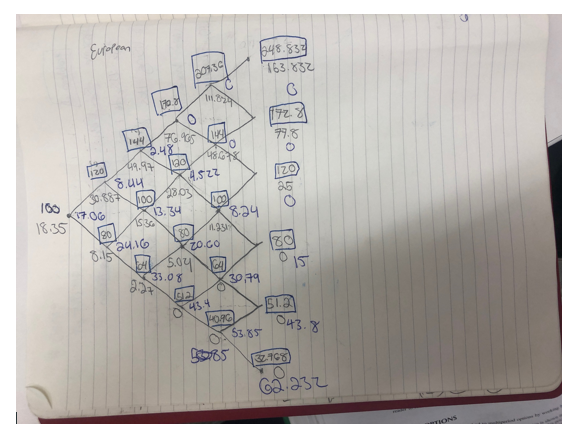
\includegraphics[width=\textwidth ]{finalp3.png}

\end{problem}

\newpage
\begin{problem}{4}. Consider Apple Inc. as the underlying asset, use its daily adjusted closing prices from August 13, 2018 to August 13, 2019 as historical data.\\
\underline{Part 1,2} See Excel Sheet.  \\
\underline{Part 3} $\sigma = 0.314, \ r=0.02, T= 12 , \ S_0 = 204.75, \ K_1 = 180, \ K_2 = 225$. \\
\underline{Def: Black Scholes Option Formulas} 
\begin{align*}
C(S,t) &= SN(d_1)-Ke^{-r(T-t)}N(d_2) \\
P(S,t) &= Ke^{-r(T-t)}N(-d_2)-SN(d_1) \\
d_1 &= \frac{ln(s/k) + (r-\sigma^2/2)(T-t)}{\sigma \sqrt{T-t}} \\
d_2 &= d_1 = \sigma \sqrt{T-t}\\
\Delta_{call} &= N(d_1) \\
\Gamma_{call} &= \frac{N'(d_1)}{S\sigma \sqrt{T-t}} \\
\Delta_{put} &= -N(-d_1) 
\end{align*}
We have 12 months so T-t is 1. I've coded all of this into R. So I will not be demonstrating the formulas step by step. For the call option: $d_1 = 0.5997, \ d_2 = 0.2857 $ these give: $N(d_1)=0.72565, \ N(d_2) = 0.6124483$.And hence, $C(S,t) =  39.067$. With $\Delta = 0.72565 $ and $\Gamma = 0.0926 $ 

For the Put option: $d_1 = -0.11092, \ d_2 = -0.42491$ these give: $N(d_1)=0.54415, \ N(d_2) = 0.6645 $. And thus, $P(S,t)=36.23531. $ With $\Delta = -0.54415 $ and $\Gamma = 0.08811015$ \\
\end{problem}

\end{document}
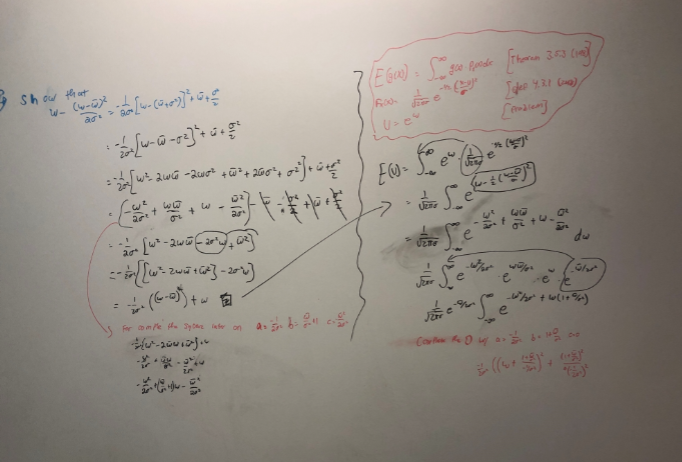
\includegraphics[width=\textwidth ]{mod10p4c.png}



% Set the overall layout of the tree




\tikzstyle{level 1}=[level distance=3.5cm, sibling distance=3.5cm]
\tikzstyle{level 2}=[level distance=3.5cm, sibling distance=2cm]

% Define styles for bags and leafs
\tikzstyle{bag} = [text width=4em, text centered]
\tikzstyle{end} = [circle, minimum width=3pt,fill, inner sep=0pt]

\begin{tikzpicture}[grow=right, sloped]
\node[bag] {Bag 1 $4W, 3B$}
    child {
        node[bag] {Bag 2 $4W, 5B$}        
            child {
                node[end, label=right:
                    {$P(W_1\cap W_2)=\frac{4}{7}\cdot\frac{4}{9}$}] {}
                edge from parent
                node[above] {$W$}
                node[below]  {$\frac{4}{9}$}
            }
            child {
                node[end, label=right:
                    {$P(W_1\cap B_2)=\frac{4}{7}\cdot\frac{5}{9}$}] {}
                edge from parent
                node[above] {$B$}
                node[below]  {$\frac{5}{9}$}
            }
            edge from parent 
            node[above] {$W$}
            node[below]  {$\frac{4}{7}$}
    }
    child {
        node[bag] {Bag 2 $3W, 6B$}        
        child {
                node[end, label=right:
                    {$P(B_1\cap W_2)=\frac{3}{7}\cdot\frac{3}{9}$}] {}
                edge from parent
                node[above] {$B$}
                node[below]  {$\frac{3}{9}$}
            }
            child {
                node[end, label=right:
                    {$P(B_1\cap B_2)=\frac{3}{7}\cdot\frac{6}{9}$}] {}
                edge from parent
                node[above] {$W$}
                node[below]  {$\frac{6}{9}$}
            }
        edge from parent         
            node[above] {$B$}
            node[below]  {$\frac{3}{7}$}
    };
\end{tikzpicture}


\section{Definitions}
\underline{Def: Forward Rate Formulas} (pg 79). The implied forward rate between times $t_1$ and $t_2$ is the rate of interset between those times that is consistent with a given spot rate curve. For Yearly compounding, the forward rate is:  
\begin{align*}
f_{i,j} =& [\frac{(1+s_j)^j}{(1+s_i)^i}]^{1/(j-i)}-1 \\
 e^{s(t_2)t_2} =& e^{s(t_1)t_1}e^{f_{t_1,t_2}(t_2-t_1)}
\end{align*}

\underline{Discount Factor Relation} The discount facot between periods i and j is defined as $$ d_{i,j}=[\frac{1}{1+f_{i,j}}]^{j-i}$$ These factors satisfy the compounding rule: $d_{i,k}=d_{i,j}d_{j,k}$\\

\underline{Def. Derivative (Ross pg 223)} Let F be a real valued function defined on an open interval contained a point a. We say f is differentiable at a, or f has derivative at a if the limit $$ f'(a) = \lim_{x \to a} \frac{f(x)-f(a)}{x-a} $$




https://www.investopedia.com/university/advancedbond/bond-pricing.asp
https://quant.stackexchange.com/questions/22288/duration-of-perpetual-bond
http://people.stern.nyu.edu/gyang/foundations/sample-final-solutions.html
http://pages.stern.nyu.edu/~jcarpen0/courses/b403333/07convexh.pdf
https://web.stanford.edu/class/msande247s/2009/summer%2009%20week%205/Bond%20Formula%20Sheet.pdf


\underline{Def: Forward Rate Formulas} (pg 79). The implied forward rate between times $t_1$ and $t_2$ is the rate of interset between those times that is consistent with a given spot rate curve. For Yearly compounding, the forward rate is:  
\begin{align*}
f_{i,j} =& [\frac{(1+s_j)^j}{(1+s_i)^i}]^{1/(j-i)}-1 \\
 e^{s(t_2)t_2} =& e^{s(t_1)t_1}e^{f_{t_1,t_2}(t_2-t_1)}
\end{align*}

\underline{Discount Factor Relation} The discount facot between periods i and j is defined as $$ d_{i,j}=[\frac{1}{1+f_{i,j}}]^{j-i}$$ These factors satisfy the compounding rule: $d_{i,k}=d_{i,j}d_{j,k}$\\

\underline{Def. Derivative (Ross pg 223)} Let F be a real valued function defined on an open interval contained a point a. We say f is differentiable at a, or f has derivative at a if the limit $$ f'(a) = \lim_{x \to a} \frac{f(x)-f(a)}{x-a} $$



\begin{align*}
\text{Maximize  } & 4x_1 +5x_2 +3x_3 +4.3x_4 + x_5 + 1.5x_6 + 2.5x_7 + 0.3x_8 + x_9 + 2x_{10} \\
\text{Subject to } & 2x_1 + 3x_2 + 1.5x_3 + 2.2x_4 +0.5x_5 +15x_6 + 2.5x_7 +0.1x_8 + 0.6x_9 + x_{10} \leq 5 \\ 
& x_1 + x_2 + x_3 + x_4 \leq 1 \\
& x_5 + x_6 + x_7 \leq 1 \\
& x_8 + x_9 + x_{10} \leq 1 \\
\end{align*}